\def\myrad{2cm}% radius of the circle
\def\myang{60}% angle for the arc

\begin{figure}[h!]
\begin{minipage}{0.3\textwidth}
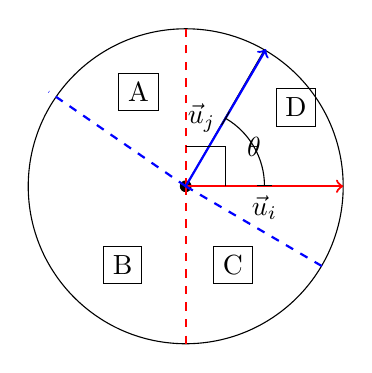
\begin{tikzpicture}
% the origin
\coordinate (O) at (0,0);
% the circle and the dot at the origin
\draw (O) node[circle,inner sep=1.5pt,fill] {} circle [radius=\myrad];
% the ``\theta'' arc
\draw
  (\myrad,0) coordinate (xcoord) -- 
  node[midway,below] {$\vec u_i$} (O) --
  (\myang:\myrad) coordinate (slcoord) 
   node[midway,left] {$\vec u_j$} (O) ;
%  pic [draw,->,angle radius=1cm] {angle = xcoord--O--slcoord};
% the outer ``s'' arc

\draw[red,thick, ->] (0,0) -- (\myrad,0);
\draw[red,thick,dashed] (0,0) -- (0, \myrad);
\draw[red,thick,dashed] (0,0) -- (0, -\myrad);

\draw[blue,thick, ->] (0,0) -- (\myrad * 0.51,\myrad * 0.87);
\draw[blue,thick,dashed] (0,0) -- (\myrad * 0.87,-\myrad * 0.51);
\draw[blue,thick,dashed] (0,0) -- (-\myrad * 0.87,\myrad * 0.6);

\node[draw] at (-0.6,1.2) {A};
\node[draw] at (-0.8,-1) {B};
\node[draw] at (0.6,-1) {C};
\node[draw] at (1.4,1) {D};

\draw (0.5,0) -- (0.5,0.5) -- (0,0.5);

\draw[|-|]
  (1,0)
  arc[start angle=0,end angle=\myang,radius=1]
    node[midway] {$\theta$};

%\draw[|-|]
%  (\myrad * 0.87,-\myrad * 0.51)
%  arc[start angle=-30,end angle=\mynty,radius=\myrad+10pt]
%    node[midway,fill=white] {$s$};
\end{tikzpicture}
\end{minipage}
\hfill
\begin{minipage}{0.55\textwidth}
\begin{enumerate}
\item Region A: $\trans{\vec r} \vec u_i \geq 0$ and $\trans{\vec r} \vec u_j < 0$
\item Region B: $\trans{\vec r} \vec u_i \geq 0$ and $\trans{\vec r} \vec u_j \geq 0$
\item Region C: $\trans{\vec r} \vec u_i < 0$ and $\trans{\vec r} \vec u_j \geq 0$
\item Region D: $\trans{\vec r} \vec u_i < 0$ and $\trans{\vec r} \vec u_j < 0$
\end{enumerate}
\end{minipage}
\caption{A random vector $\vec r$ can lie in any of the four regions. Region A (resp. C) cover $\frac{\theta}{2 \pi}$ of the area. The probability that $i \in S$ and $j \notin S$ is equal to the area of region A.}
\label{fig:angleanalysis}
\end{figure}